\documentclass[a4paper,man,natbib,floatsintext,12pt]{apa7}

\usepackage[english]{babel} %character and hyphenation rules specific to the language you choose
%\usepackage[utf8x]{inputenc}
\usepackage{graphicx}
\usepackage{color}
\usepackage{tikz}
\usepackage{amsmath}
\usepackage{blindtext}
\usepackage{tabularx} %great for APA-style Tables
\usepackage{siunitx} % Required for good table ali gnmen
\usepackage{threeparttable}

\sisetup{
  round-mode          = places, % Rounds numbers
  round-precision     = 2, % to 2 places
}
\usepackage{multirow}
\usepackage{booktabs}
\usepackage{wrapfig}
\usetikzlibrary{shapes,decorations,arrows,calc,arrows.meta,fit,positioning}
\tikzset{
    -Latex,auto,node distance =1 cm and 1 cm,semithick,
    latent/.style ={ellipse, draw, minimum width = 0.7 cm},
    observed/.style ={rectangle, draw},
    bidirected/.style={Latex-Latex,dashed},
    el/.style = {inner sep=2pt, align=left, sloped}
}
\newcommand{\sigFtest}[4]{\textit{F}(#1,#2) = #3, \textit{p}$<$#4}
\newcommand{\nonsigFtest}[3]{\textit{F}(#1,#2) = #3, \textit{p}$>$.05}


\title{ Laugh with family or strangers? Explore the role of social connectedness in the perception of laughter contagion  }
\shorttitle{Laughter Contagion}
\author{Sarah Liu}
\authorsaffiliations{College of William \& Mary}
\journal{Laughter Journal}

\abstract{\blindtext}
\keywords{APA style, demonstration}
\authornote{Thanks for my cat helping me write this paper}

\leftheader{Alternate page header in man mode}

%-------------- END PREAMBLE  -------------------


\begin{document}

\maketitle  %Insert my APA style title page

\section{Introduction}

Laughter is a universal non-verbal vocalization that conveys positive emotions in human interaction \citep {sauter2010cross, scott2014social}.  The social nature of laughter is also evident by the finding that people are up to 30 times more likely to laugh when with others than when alone \citep{provine1989laughing}.

\subsection{Social connectedness and laughter contagion}
The behaviourally contagious phenomenon is strongly mediated by social bonding, especially the level of connectedness between a \textit{laugher} (person who produces the laughter) and a \textit{listener} (person who receives the laughter): people are more likely to laugh in response to a friend's laughter than to a stranger's \citep{smoski2003antiphonal}.

\subsection{Current Research}

The primary aim of the current research was to investigate how social connectedness between the laughers and listeners affects the perception of laughter contagion. Using spontaneous laughter recordings from 17 interconnected individuals (including friends and family members) collected in 2012, we invited this acquaintance group again to the study and listened to each other’s laughter recording (including laughter from themselves) in a laughter perception task. After listening to each laughter recording, they rated the contagiousness and the social connectedness with the laugher. Furthermore, we manipulated an informing effect, that is, whether participants were presented with the laugher’s name before listening to the recording. Based on the relationship between social connectedness, informing condition, and contagion rating, we predicted that:

\begin{enumerate}
    \item  \textit{Hypothesis 1} (H1) — Strength of Social Connectedness: listeners would experience more contagious laughter when they feel more socially connected with the laugher. 
    \item  \textit{Hypothesis 2}  (H2) — Informing of Laughter’s identity: presenting the names of the laughers before participants listen to the recording would result in a stronger contagious effect.
    \item  \textit{Hypothesis 3}  (H3) — Interaction Effect: An interaction effect between social connectedness and informing effects, such that the impact of social connectedness on laughter contagion may depend on prior informing of the laugher’s identity.
\end{enumerate}

\section{Method}
\subsection{Participants}
The study has been approved by the PaLS - Institute of Cognitive Neuroscience/ BUCNI LREC as Project ID 0210. For the acquaintance group, 17 interconnected participants who provided their laughter recordings in 2012 were contacted again, and 10 of them responded and completed the experiment. Seven additional family members/friends of these laughers were recruited through a snowball sampling technique (referred by laughers). The final acquaintance group of 17 participants consisted of 10 females and 7 males, between the ages of 18 and 61 (\textit{M }= 41.29, \textit{SD} = 16.81).

\subsection{Materials}
The experiment was built and conducted on the Gorilla (https://gorilla.sc/), an online experiment builder platform \citep {anwyl2020gorilla}. Participants completed the task on their personal computers and headphones.

\subsubsection{Laughter Perception Task (LPT)}

LPT consisted of two blocks. Both blocks involved listening to recordings of laughter. 68 spontaneous laughter recordings were collected from 17 laughers (7 females and 10 males) in 2012. While these participants were shown funny YouTube videos, their natural responses were recorded in an Anechoic chamber. Each laugher contributed two recordings per block.

In Block 1, participants were not informed of the names of laughers in the recording. After listening to each recording, they were asked to 1) rate the contagion (“How much does this laughter make you laugh”) on a scale from 1, meaning “I don’t want to laugh at all,” to 10 “I laugh a lot.” 2) rate the familiarity (“does this laughter sound familiar?”) on a scale from 1, meaning “not familiar,” to 10, “very familiar” (Figure 1). In order to ensure participants focused on the task, three vigilance trials were also applied in random order, in which participants were asked to select the number that the speaker in the audio said. A total of 37 trials ( 34 laughter perception trials and 3 vigilance trials) were conducted.

In Block 2, before listening to the laughter recording, participants in the acquaintance group were presented with the laugher’s name, a manipulation reffered to as the informing effect. After listening to each recording, they were again asked to rate the contagiousness of laughter on the same scale as above. Differently, this time, they were asked to judge their closeness with the laugher (“Is this person close to you?”) instead of familiarity, on a scale from 1 “not close” to 10 “very close” (see Figure~\ref{fig1}). Three vigilance trials were applied. A total of 37 trials ( 34 laughter perception trials and 3 vigilance trials) were conducted.

\begin{figure}[h!] 
\centering
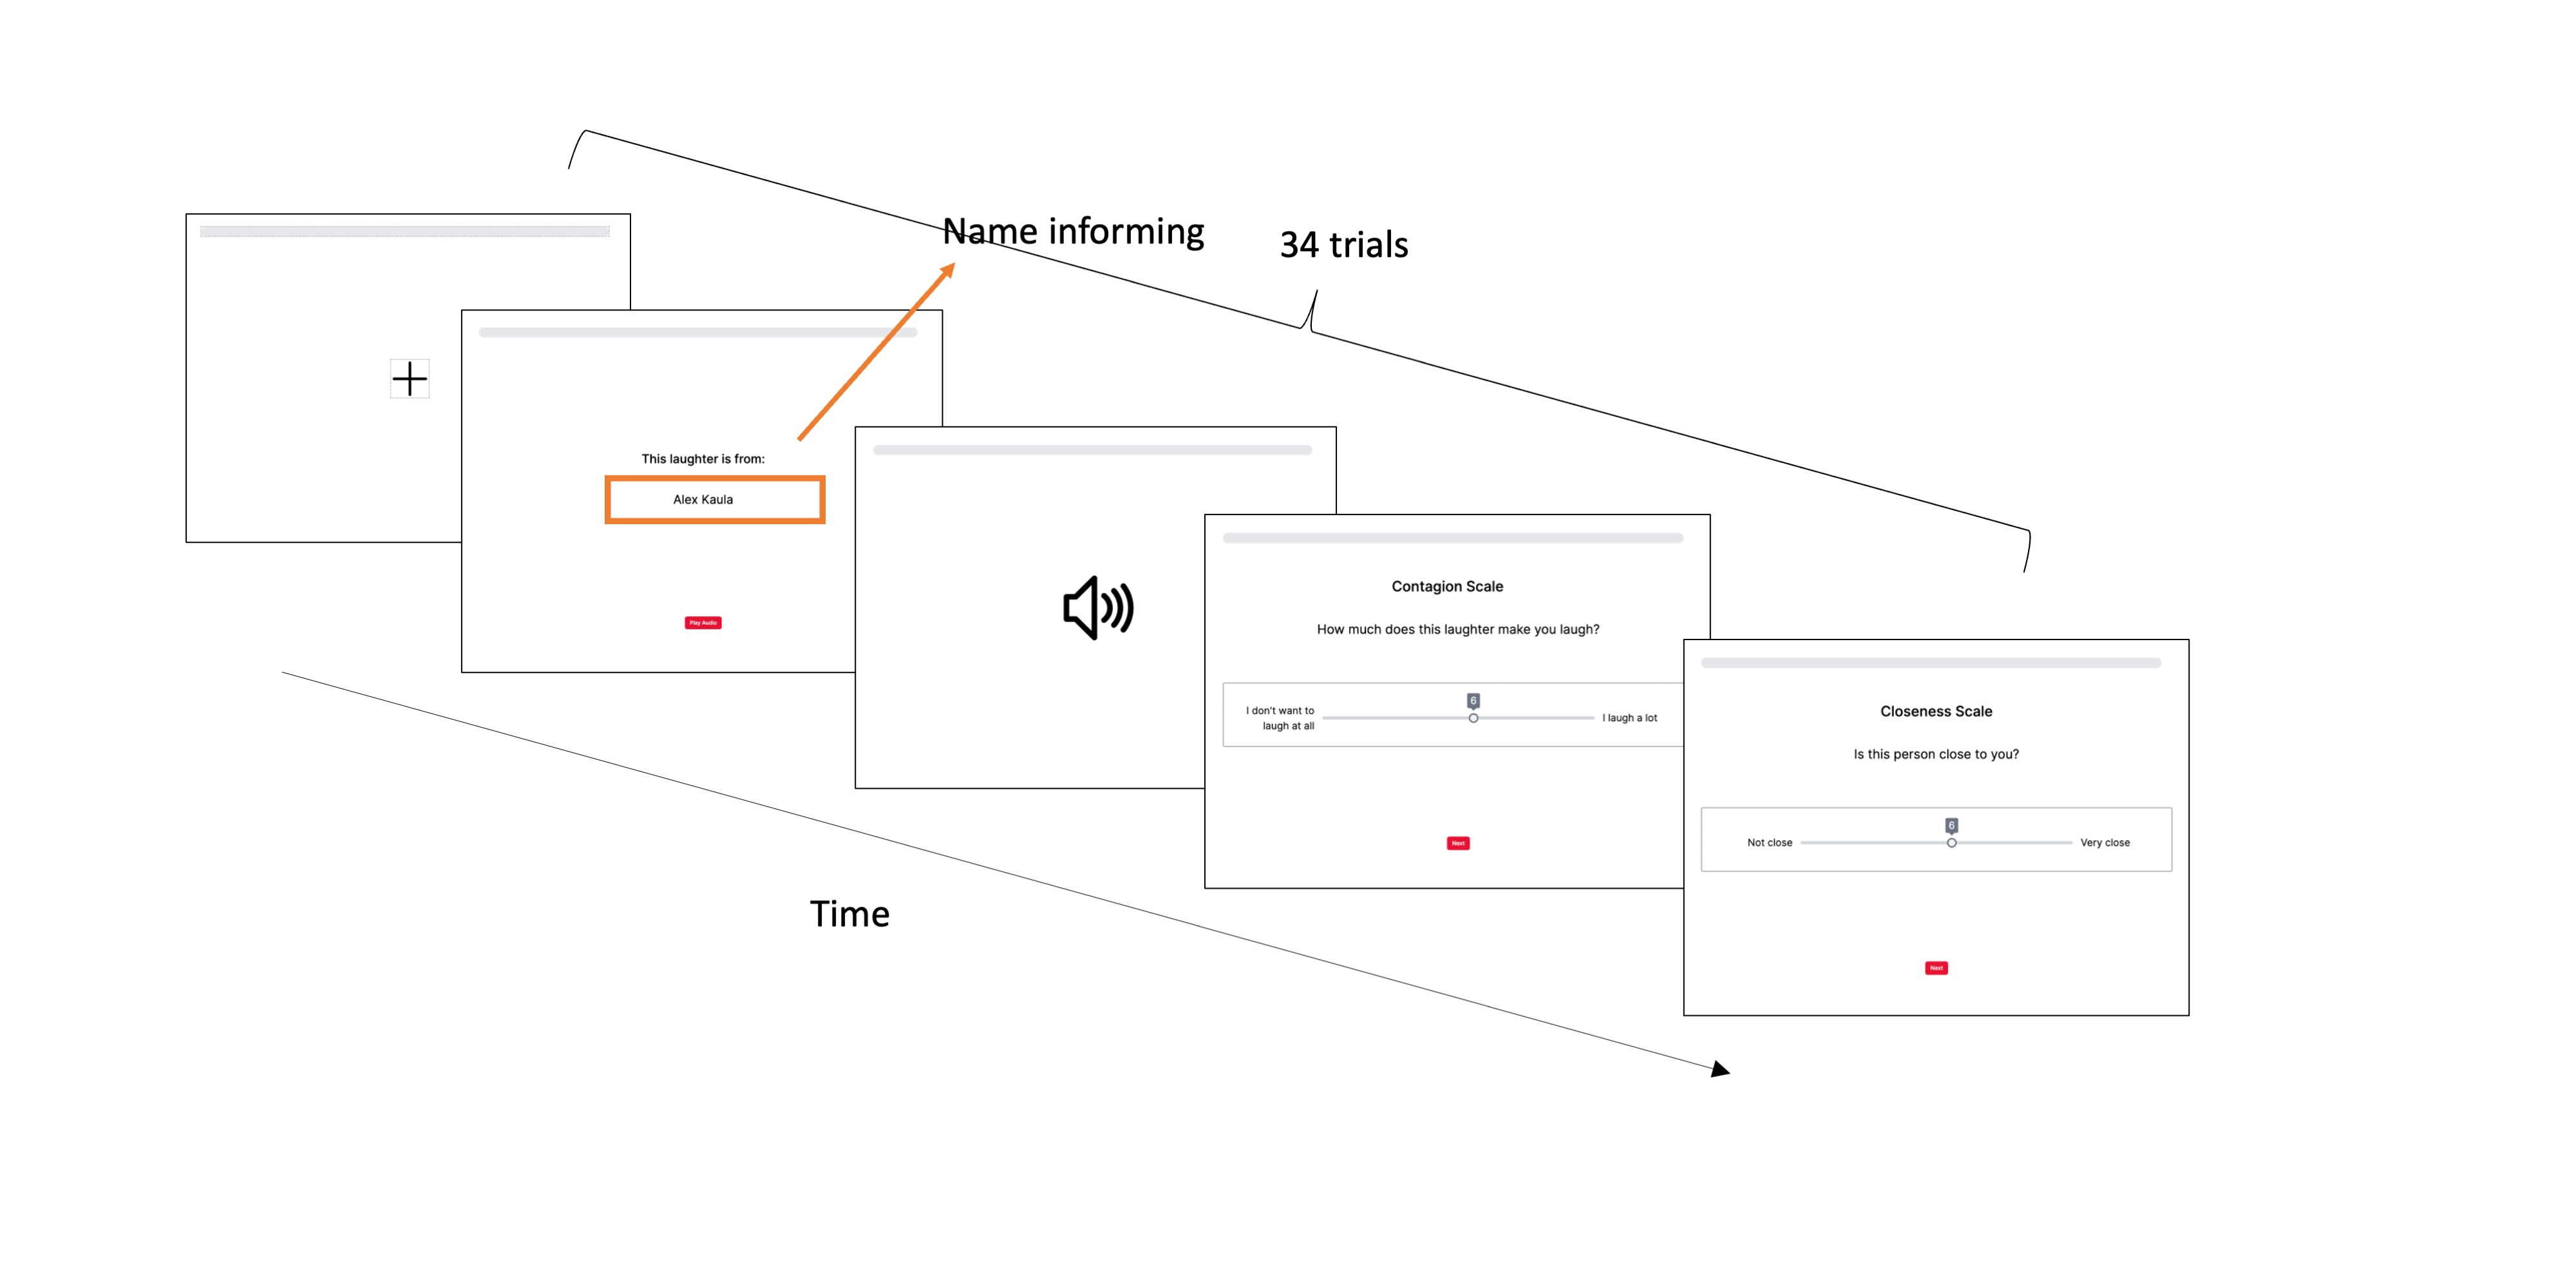
\includegraphics[width=1\textwidth]{Slide2.jpeg}
\caption{\label{fig1}Laughter Perception Block 1 Illustration.}
\end{figure}

In Block 2, before listening to the laughter recording, participants in the acquaintance group were presented with the laugher’s name, a manipulation referred to as the informing effect. After listening to each recording, they were again asked to rate the contagiousness of laughter on the same scale as above. Differently, this time, they were asked to judge their closeness with the laugher (“Is this person close to you?”) instead of familiarity, on a scale from 1 “not close” to 10 “very close”(Figure ~\ref{fig2}). Three vigilance trials were applied. A total of 37 trials ( 34 laughter perception trials and 3 vigilance trials) were conducted.

The stranger group received the same task format as Block 1. As we assumed participants from the stranger group may not personally know the laughers in the recordings, providing the laughers’ names would not affect their performance in general, and therefore, there was no name-informing procedure for the stranger group in Block 2.

\begin{figure}[h!] 
\centering
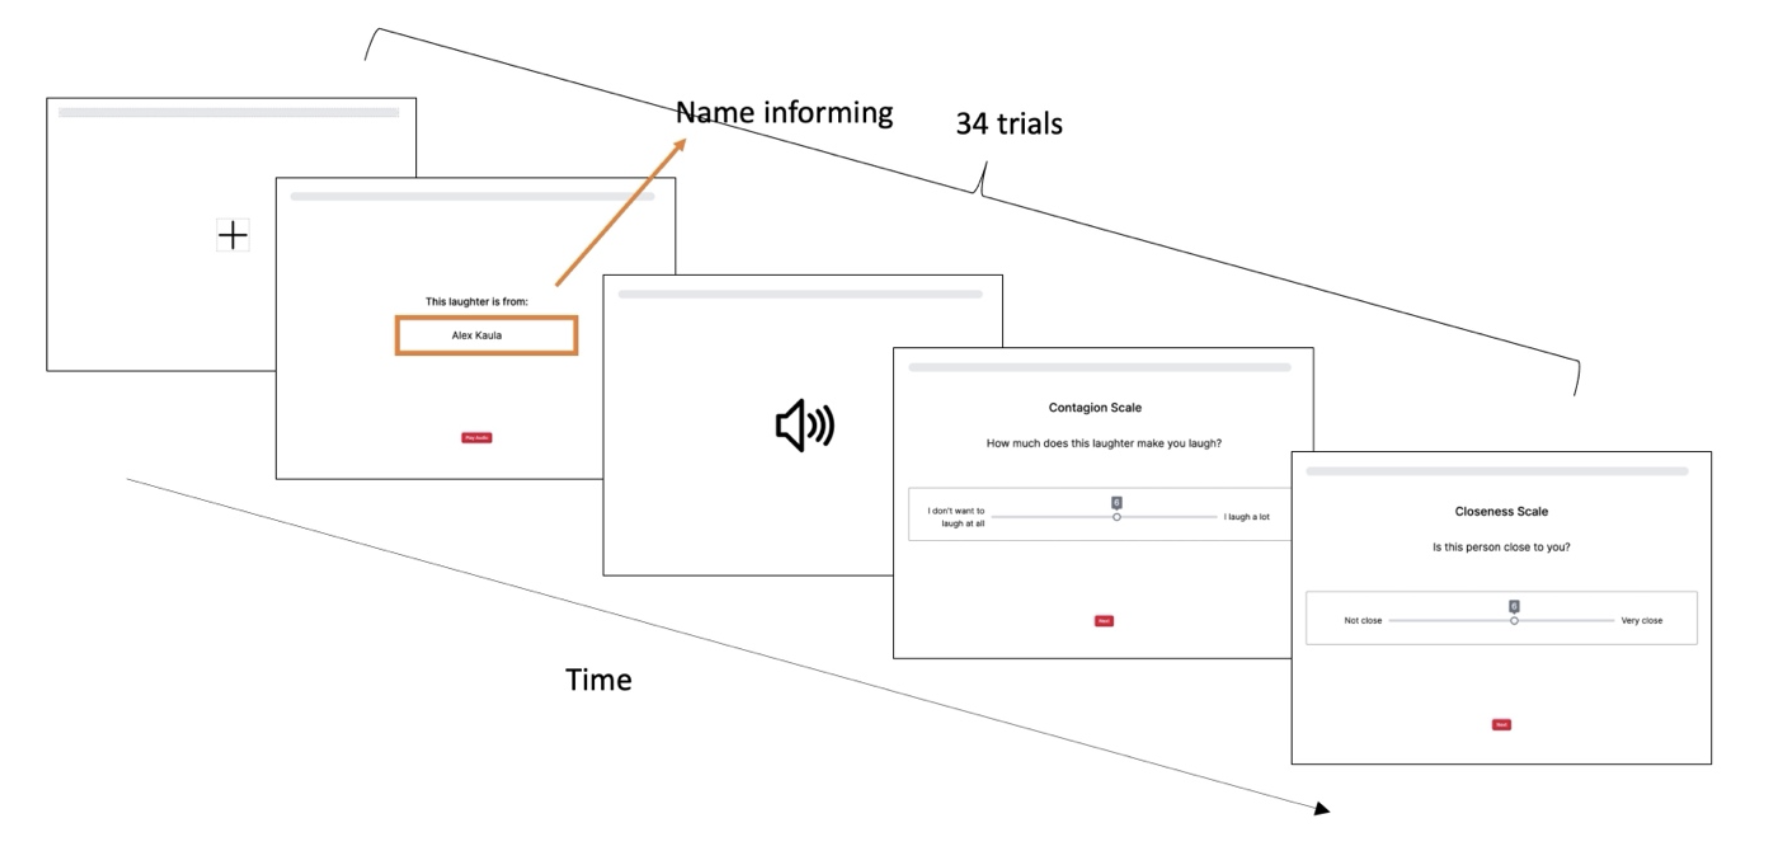
\includegraphics[width=13cm]{Screenshot 2025-09-03 at 11.29.56.png}
\caption{\label{fig2}Laughter Perception Block 2 Illustration.}
\end{figure}


\subsection{Procedure}
Participants in the acquaintance group were invited to the Gorilla online experiment through an email link; the stranger group was invited through Prolific. After providing informed consent, participants completed a sound check to ensure the audio devices were connected.

Participants were first asked to provide demographic information (age, gender, sex) and then completed two questionnaires (LSAS and LPPQ).

\subsection{Statistical analyses}
 For the primary research question (H1 – H3), we were interested in the effect of social connectedness on laughter contagion at different manipulations. Only data from acquaintance groups (\textit{n} = 17) were used, as we assume that the stranger group does not experience social effects. To account for variations within individuals and items, we built a Linear Mixed-effects Model using the lmer function from the lmer4 package (Bates et al., 2015) in R (version 4.4.1). Fixed effects consisted of the social connectedness effect, informing effect, and their interaction. For random effects, we started with the maximal structure with the item and the participant intercepts and slopes (Barr et al., 2013), but not all models converge with this structure. In order to ensure the model converges, we selected a maximal random structure that consisted of by-participants (ID) random slopes and intercepts and by-item intercepts only. This random effect structure accounted for individual differences (individual propensity to laughter contagion and fixed effects) and item differences (variations in contagion level across each laughter recording). Overall, the use of a Linear Mixed-effects Model allowed us to assess the impact of the predictor and manipulation on changes in the outcome variables. The estimates in the mixed-effects model represented the estimated effect size. Statistical significance was set at p <0.05. 

\section{Results}
\subsection{Descriptive statistics}
Descriptive statistics, including the mean and standard deviation of connectedness rating and contagion rating across two conditions of informing, are presented in Table \ref{tab:table1}. Together with Figure 5, when no names of laughter were given before listening to the recordings (i.e., uninformed condition), the social connectedness ratings predicted a linear relationship with the contagion rating. In contrast, when the name was given (i.e. informed condition), there was a boost effect for contagion ratings at lower social connectedness ratings.



\begin{table}[h!]
\centering
\begin{threeparttable}
\caption{Descriptive statistics for primary analysis.}
\label{tab:table1}
\begin{tabular}{l l c c c c} 
    \toprule
    & & \multicolumn{2}{c}{Contagion} & \multicolumn{2}{c}{Connectedness}  \\ \cmidrule{3-6}
    & & \textit{M} & \textit{SD} & \textit{M} & \textit{SD}   \\ \cmidrule{3-6}
    \multirow{ 2}{*}{Informing} & Yes & 5.855 & 6.76 & 9.1 & 2.69 \\ & No & 6.23 & 1.67 & 02.23 &5.3 \\
      \bottomrule
\end{tabular}
\begin{tablenotes}
\small
\textit{Note}. \textit{M} = mean; \textit{SD} = standard deviation.
\end{tablenotes}
\end{threeparttable}
\end{table}



\section{Discussion}
\subsection{Summary of main result}
In the current study, we investigated social dynamics in the perception of laughter contagion. To answer this primary research question, we examined whether laughter recordings from more socially connected individuals would be rated as more contagious. Results supported the hypothesized main effect of social connectedness: without any additional context, when people listened to the laughter from more familiar or closer individuals, they experienced a stronger contagious effect. This result aligns with the previous research suggesting that social bonding mediates laughter perception \citep{smoski2003antiphonal}. Importantly, our study extends this line of research by examining a variety of interpersonal relationships (e.g., friends, couples, relatives), contributing to a broader understanding of how social bonding influences the contagiousness of laughter.

We also found a significant informing effect consistent with Hypothesis 2: when participants were given the laugher’s name before listening to the recording, participants perceived the laughter as more contagious than when no name was given. In addition, the significant interaction effect (Hypothesis 3) found that the social connectedness effect was less pronounced in the informed condition. When no information regarding the laughter’s identity was presented, social connectedness showed a linear relationship with the contagion ratings; when informing was applied, contagion ratings were slightly higher overall. To further examine the social effect, in the exploratory analysis, we found that self-laugher was perceived to be more contagious than others’ laughter, regardless of whether participants were informed of the laugher’s identity.

\subsection{Conclusion}
Our study provides new insights into how social connectedness modulates the perception of contagious laughter. We found a social asymmetry underlying the contagion perception and the emotion transfer process. The sense of familiarity created by the mere exposure of the laugher’s name could enhance the contagion perception. In addition, we presented the first evidence that individuals perceive self-laughter as more contagious than others’ laughter, which could also be due to familiarity with oneself. Together, our study lays the ground for the potential of using laughter as a valuable proxy to elucidate socio-emotion dynamics.

Lastly, we revealed individual differences in the perception of laughter contagion. People with impoverished social bonding still experience a comparable level of laughter contagion. Individual differences in Frequency, Liking, and Usage of laughter measured from LPPQ are also closely associated with the contagion rating, which establishes the applicability of the Laughter Production and Perception Questionnaire (LPPQ) to understand the considerable variations in human laughing behaviors.
\bibliography{reference}



\end{document}